\chapter{Implementation\label{cha:chapter5}}

This chapter describes the implementation of component X. Three systems were chosen as reference implementations: a desktop version for Windows and Linux PCs, a Windows Mobile version for Pocket PCs and a mobile version based on Android.

\section{Environment\label{sec:env}}
The following software, respectively operating systems, were used for the implementation:

\begin{itemize}
		\item Windows XP and Ubuntu 6
		\vspace{-0.1in}
		\item Java Development Kit (JDK) 6 Update 10
		\vspace{-0.1in}
		\item Eclipse Ganymede 3.4
		\vspace{-0.1in}
		\item Standard Widget Toolkit 3.4
\end{itemize}

\section{Project Structure\label{sec:projectstructure}}

The implementation is seperated into 2 distinguished eclipse projects as depicted in figure \ref{fig:projects}.

\begin{figure}[htb]
  \centering
  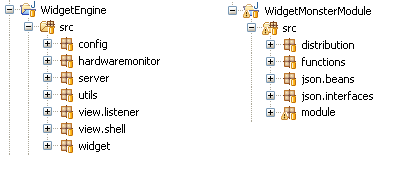
\includegraphics[width=10cm]{screenshot_2_projects}
  \caption{Project Structure}
  \label{fig:projects}
\end{figure}

\noindent
The following listing briefly describes the single packages of both projects in alphabetical order to give an overview of the implementation:
\\
\\
\textbf{config}
\\
Lorem Ipsum...
\\
\\
\textbf{server}
\\
Lorem Ipsum...
\\
\\
\textbf{utils}
\\
Lorem Ipsum...

\section{Important Implementation Aspects\label{sec:gui}}

Do not explain every class in detail. Give a short introduction about the modules or the eclipse projects. If you want to explain relevant code snippets use the 'lstlisting' tag of LaTeX. Put only short snippets into your thesis. Long listing should be part of the annex.

\lstset{caption=JSON String Code Snippet,label=jsonstring,showstringspaces=false}
\begin{lstlisting}
{
	id: 1,
	method: "myInstance.getGroup",
	params: ["Teammates", 2, true]
}

{
	id: 2,
	result: [
		  "groupDesc":"These are my teammates",
		  {
			"javaClass":"src.package.MemberClass",
			"memberName": "Bob",
		  }
		]
}\end{lstlisting}

You can also compare different approaches. Example: Since the implementation based on X failed I choosed to implement the same aspect based on Y. The new approach resulted in a much faster ...

\section{Graphical User Interface\label{sec:gui}}

Lorem Ipsum...

\section{Documentation\label{sec:docu}}

Lorem Ipsum...
